\documentclass[a4paper,12pt]{report}

%packages
\usepackage[utf8]{inputenc}
\usepackage{mathtools}
\usepackage{amsfonts}
\usepackage[onehalfspacing]{setspace}
\usepackage{graphicx}
\usepackage{caption}
\usepackage{subcaption}

%document
\begin{document}
\begin{titlepage} 
  \parindent0pt 
  \hskip.25cm \vrule width.8pt \hskip.25cm 
  \begin{minipage}{\dimexpr\linewidth*2-2.5cm-.8pt-2.5cm\relax} 
    \sffamily\bfseries {
    \huge Master 2 Bioinformatique\par}\large 
    Semestre 10\par Université de Bordeaux\par 
    %%Année truc
  \end{minipage}%
  \vskip10pt plus 1fil
  \fbox{%
  \begin{minipage}{\dimexpr\linewidth-2\fboxsep-2\fboxrule} 
    \centering\Large\bfseries 
    \vskip1cm 
    Project report: TITLE\par 
    \vskip1cm \kern0pt 
  \end{minipage}%
  }%
  \vskip0.5cm 
  {\centering 
  \vskip0pt plus 1fil 
  }%

  \textbf{Aurélien \sc{Luciani}}\centering\\ 
  \vskip0pt plus 1fil 
  \hfill \hskip.25cm \vrule width.8pt \hskip.25cm 
  \vskip0pt plus 1fil {\centering Supervisor\,: Murray P. \sc{Cox} \par }
  \vskip0pt plus 2fil 
  \hfill\bfseries{Year 2014-2015}\hfill\null 
\end{titlepage}

% to be removed...
%\setcounter{tocdepth}{1}
% ...until here
\begin{spacing}{1.2}
 \tableofcontents
\end{spacing}
%\addtocontents{toc}{\protect\enlargethispage{\baselineskip}}

\chapter*{Introduction}
\addcontentsline{toc}{chapter}{Introduction}
Two groups of populations can be identified in the Islands of South-East Asia (ISEA), one is composed of the Melanesians, whose ancestors settled in these islands during the first human settlement, around 45 thousand years ago. The other arrived more recently during a period often called the Austronesian expansion, between 5 and 4 thousand years ago, when people from mainland China settled in the islands. Nowadays people living in this area have mixed genomic ancestry and markers can be identified and defined as either from an Asian ancestry or a Melanesian one. These markers are based on signle nucleotid polymorphisms located in different chromosomes and 52 markers can be used to define accurately the admixture of the Asian ancestry in every individuals \cite{Cox01}.

The choice of these SNPs is a result of previous studies at Massey University, the University of Arizona, the Santa Fe Institute, and the Eijkman Institute that sequenced 1430 individuals from 60 populations. This set of SNPs is defined as highly informative and allows to define the ancestry of a person based on a small quantity of markers that are highly discriminant.

Two specific patterns can be seen, one is the non linear gradient of Asian admixture when observing individuals in the different islands when looking along the longitudinal axis, corresponding more or less the wave the settling might have happened. The second is the difference of admixture when looking at specific parts of the genomes associated with male or female ancestry, implying a gender-biased expansion.
% first papers
% whole project for the group
%% leading to the creation of the model


\chapter{Project presentation}
The project consists of developing a model of the Austronesian expansion throughout the ISEA that could reproduce the same two patterns observed in the real data.
The first pattern can be seen in the figure (REF!!!) and is a non-linear gradient in Asian admixture that declines abruptly around the eastern part of Indonesia. The second one, represented in the figure (REF!!!), is a 

\section{Type of values observed}

\section{Model used}

\begin{figure}
	\centering
	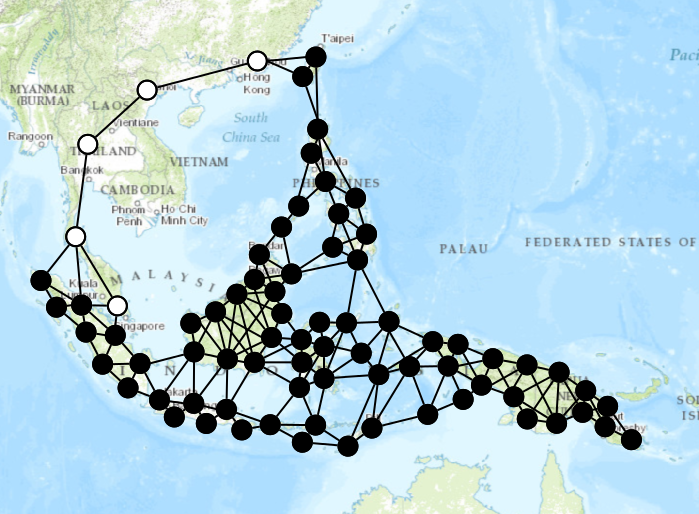
\includegraphics[scale=0.55]{../data/nodesOnMap.png}
	\caption{Nodes of a model superimposed on the map of the modelled region. White nodes are the Asian nodes at the beginning of the simulation and the black ones are the Melanesian ones}
	\label{nodesOnMap}
\end{figure}

Because of the stochasticity of the models, a simulation can have non-usable outputs. For example, if an island end up being completely empty, the admixture values yielded by this specific simulation will be \texttt{NaN} (not a number). In such extreme cases, the model can be considered as failed and can either be discarded or given the worst possible score, depending on the current analysis. Arbitrarily, rules have been set to define a simulation as failed:
\begin{itemize}
	\item If a deme has a population of less than 10\% of the most populous deme in the network, it is considered as empty;
	\item If more than 25\% of the demes in any of the islands are empty, the model is considered as failed.
\end{itemize}

\subsubsection{Comparison to other models}
\subsubsection{Parameters}

\begin{table}
	\centering
	\begin{tabular}{|c|c|c|c|}
		\hline
 		Parameter & Values & Estimated & Comment \\ \hline
        Migration probability & $\mathbb{R}_{0 \leq x \leq 1}$ & $\mathbb{R}_{0 < x \leq 0.8}$ & probability to start migrating \\ \hline
        Starting distribution & \{...\} & \{...\} & starting admixtures \\ \hline
        Fecundity & $\mathbb{R}_{\geq 0}$ & $\mathbb{R}_{2.3 < x < 6}$ & Poisson law mean \\ \hline
        Number of agents & $\mathbb{Z}_{\geq 0}$ & $\mathbb{Z}_{50 < x < 400}$ & population in each deme, initially \\ \hline
        Graph & \{...\} & \{...\} & graph nodes and edges \\ \hline
        Growth rate & $\mathbb{R}_{0 \leq x \leq 1}$ & $\mathbb{R}_{0 < x < 0.001}$ & limiting rate of population growth \\ \hline
        Model rules & \{...\} & \{...\} & mainly, marriages rules \\ \hline
        Marriage threshold & $\mathbb{R}_{0 \leq x \leq 1}$ & $\mathbb{R}_{0 < x < 0.5}$ & affects marriages rules \\ \hline
	\end{tabular}
	\caption{changing parameters of the model}
	\label{parameters}
\end{table}
% model details
% previous works
%% previous models
%% previous analyses

\section{Statistical analysis framework}
\subsubsection{Previous works}
\subsubsection{Specific needs}


\chapter{Implementation}
% or "realisation", "analysis pipeline"

% run management (local, cluster, NeSI)
\section{Run management}
The fact that many simulations are required to be able to infer meaningful information from the model imply that they cannot be run on a single desktop computer. In fact, running them in a single computer, the time to run enough simulations to be statistically relevant could be counted in years.
Luckily, every simulation being independent from the others, there are multiple ways to generate more results in less time.
Firstly, since nowadays most of the computers have multiple processors, one computer can run multiple simulation concurrently. Also, a cluster of computers can be used and the wanted simulations can be dispatched among the nodes of the cluster so that they each run the simulations they were assigned and when all the nodes have ended their runs, their outputs can be aggregated and/or stored.

Different levels have been used. First, running the simulations locally (figure \ref{network:local}), on a single computer, then using the three computers in the office has a cluster of compute nodes (figure \ref{network:office}), for more heavy batches. Also, since Massey University just made an agreement with Microsoft Azure, that provides computing "in the cloud", simulations have been run adding virtual machines on the Microsoft Azure system to the cluster of computers in the office transparently (figure \ref{network:azure}).
Finally, when the computation requirements were to high, for really huge batches, the NeSI\footnote{New Zealand eScience Infrastructure}'s High Performance Computing (HPC) facilities have been used (figure \ref{network:nesi}). They provide servers specially designed for scientific computation and can be tasked with hundred of parallel jobs at a time. Each node is an IBM Power755 machine.

The most powerful level used for this study is obviously using the HPC but a trade-off of using this system is that, since it is shared by multiple users and is managed by a third-party, it requires specific settings and it cannot be used exactly as can be a custom cluster of computers. The batches have to be submitted to a load leveller to the system and thus slight changes have been made to the way the model and the Repast framework are launched. Runs ran on this HPC used several nodes (usually around 4) with each 32 threads available for the simulations. This configuration leads to the parallel simulation more than a hundred of scenarios at the same time.

\begin{figure}
	\centering
	\begin{subfigure}[t]{0.48\textwidth}
		\centering
		
\includegraphics[scale=0.6]{../data/network:local.png}
		\caption{local}
		\label{network:local}
	\end{subfigure}
	~
	\begin{subfigure}[t]{0.48\textwidth}
		\centering
		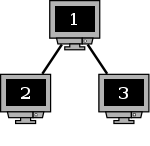
\includegraphics[scale=0.6]{../data/network:office.png}
		\caption{local network}
		\label{network:office}
	\end{subfigure}
	\\
	\begin{subfigure}[t]{0.48\textwidth}
		\centering
		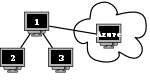
\includegraphics[scale=1]{../data/network:azure.png}
		\caption{local network and Azure}
		\label{network:azure}
	\end{subfigure}
	~
	\begin{subfigure}[t]{0.48\textwidth}
		\centering
		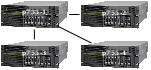
\includegraphics[scale=1]{../data/network:nesi.png}
		\caption{NeSI}
		\label{network:nesi}
	\end{subfigure}
	\caption{Different set-ups to run the model}
	\label{network}
\end{figure}

% data processing from model output
% data storage, adding and querying data
\section{Data processing, storage and query}
Since running a lot of simulations, with a lot of different parameters, can generate a lot of output files whose original parameters can be hard to track, a way to keep them organised was needed. Doing so, it would also be possible to use results from different batches and to analyse them together, thus avoiding to redo simulations for parameters already tested.

The organised way to store this is naturally in a database. The choice has been made to use a relational database, specifically MariaDB (a fork of Oracle's MySQL). The structure has been designed so that the parameters can be efficiently queried. The tables and relations between them can be seen in the figure \ref{db}. It has first been developed and tested locally and then, once it was working properly, it was deployed on a server provided by Massey University for research purposes.

\begin{figure}
	\centering
	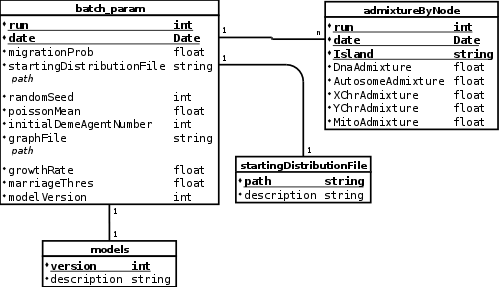
\includegraphics[scale=0.8]{../data/DB.png}
	\caption{Structure of the database storing the results of the simulations and the corresponding parameters}
	\label{db}
\end{figure}

The interaction with the database can be done through phpMyAdmin but 2 scripts have been done to interact with it, one that adds the model outputs to the database and an other one that queries the database. The scripts have been written in Python3, using the PyMySQL module to access the MariaDB database, and internally using an other script, in R, that treats the data before adding them to the DB.


\section{Analysis}


\subsection{Comparisons}
To be able to compare two different scenarios, one has to define comparison functions that will be able to provide a value of similarity or dissimilarity when provided with observable values that characterise the scenarios. In this case, the comparison is done between the real observed data and the output of one simulation.
Every simulation output has to be treated to be of the same form than the observed data so that it can be compared. The observed data does not include values for specific islands that are included in the simulations, namely Alor, Tanimbar and Aru in eastern Indonesia. The admixture values for mitochondrion and Y-chromosome are also not available for every island.
Those values in the models can then be dropped as they cannot be compared.

Many different comparison functions have been tested. Two functions have been selected that can hold different information about a comparison. The mean square distance (MSD) and the partial Mantel test have been selected as they do not have a good correlation when applying them to random admixture values, meaning that they do not carry the same information, they are complementary, and using them both gives a better overview of the comparison.

\subsubsection{Mean square distance}
The mean square distance is the mean value of all the distances between values of admixture for every $n$ island.

\begin{equation}
MSD = \frac{\sum\limits_{i=1}^{n} \sqrt{(AdReal_i - AdSim_i) ^ 2}}{n}
\end{equation}
where $AdReal$ is the array of admixture data observed in the real values and $AdSim$ the corresponding values in the simulated model.

It gives a distance value, with 0 meaning that the two observed values are absolutely identical. In this specific context, with the fact that an admixture value is compared and because of the values observed in the real data, the higher possible value will be around $0.8$.


\subsubsection{Partial Mantel test}
The Mantel test has been developed to be able to compare two matrices with the same information, the partial version of this test also uses a third matrix, holding geographical distances for the cells of the matrices to be able to weight the values according to the actual geographical distance of the points \cite{Smo01}.

In this case, the matrices contain the values of distances of admixtures between every islands in the graph and a matrix $M$ is calculated as
\begin{equation}
	M = \begin{bmatrix}
		d(Ad_0, Ad_0)	& \cdots & d(Ad_0, Ad_n) \\
		\vdots			& \ddots & \vdots		 \\
		d(Ad_n, Ad_0)	& \cdots & d(Ad_n, Ad_n)
	\end{bmatrix}
\end{equation}
were $d$ is the function returning the distance between the two arguments and $A$ the admixtures of the $n$ islands of the graph. With the corresponding matrices for the simulation data, the real data and also the geographical distances, the partial Mantel test can be done as such
\begin{equation}
	correlation = partial.Mantel(M_{Simulated}, M_{Real}, M_{geographical})
\end{equation}

the partial Mantel test returns a correlation value that is between -1 and 1 with a value of 0 meaning that the two matrices are not correlated at all and 1 that they are completely correlated.

\subsection{Visualisations}

% ABC framework



\chapter{Results}
\section{Grid search analysis}

\subsubsection{Stability analysis}


\subsubsection{Sensitivity analysis}


\section{ABC Framework}

\subsection{Priors definition}


\subsection{Posterior distribution}




\chapter{Discussion}

\section{Importance of randomness}
One important aspect that has been discovered while working with the Repast framework was the way it handles randomness. For a stochastic simulation, randomness is key, as starting two simulations with the same random seed and the same parameters would lead to the same succession of events in the simulation and thus to the same outcome. These two simulations would actually be the same one.

When looking at the results with a statistical point of view, one cannot use two identical simulations as two distinct values, that would simply make no sense and lead to biased interpretations of the values.

The problem with Repast is that it uses the current time to generate a random seed. While this can be acceptable when the program is run in one thread on a single computer, since the time at which one simulation will always be different from one other simulation, it leads to problems if the simulations are run in parallel using multiple threads on the same machine and/or using different machines and they happen to start at the same time. The risk of both the random seed and the parameter set used for the simulations colliding, while not probable, is still possible thus not acceptable. Actually, even though the random seed is supposed to be a 32 bits signed integer, meaning that there are more that 4 billions possibilities, collisions happened more than once during this project.

The first way to handle this has been to alert the user when this happened, letting him remove the specific simulations if needed. Secondly, a way has been found to generate the random seeds beforehand using Unix's random source, \texttt{/dev/urandom/}, that can generate pseudo-random values that can be used for cryptographic purposes, meaning that it is good enough to avoid collision.

% optimisations
\section{Optimisations}
Some key steps in the analysis framework need to be efficient enough so that time is not lost waiting for results to be treated or for graphs to be plotted and that the computation can be done without needing a computer.
This project has seen a few important refactoring processes to be able to cope with the quantity of data to be treated. The most important have been to treat the simulation results as a stream of values instead of loading the whole dataset in memory. This changed the memory complexity from linear to constant and it actually improved the time complexity from sub-quadratic to linear for the treatment part and from sub-quadratic to linearithmic for the analysis part. The improvement in time has been made possible by assuming that the results of one simulation are always together in the result stream, that way saving the cost of searching results in a big block of memory when they are actually next to each other.
Actual execution times have been recorded and can be seen in the graph (REF!!!).\

The stream approach also allows the different steps of an analysis to be run simultaneously, by piping each step to the next, effectively making the whole process run in parallel. This is useful only if the computer used has at least $n$ cores if $n$ processes need to be run in parallel. In this case, the time of the whole process is the time needed to run the longest step.


% other visualisations
\section{Other visualizations}
% more complex model
\section{More complex model}


\chapter*{Conclusion}
\addcontentsline{toc}{chapter}{Conclusion}

\bibliography{main}
\bibliographystyle{apalike}

\appendix
\addtocontents{toc}{\protect\setcounter{tocdepth}{-1}}
% example visualisations
%\addtocontents{toc}{\setcounter{tocdepth}{-1}}
\chapter{Examples of visualisation}
%\addtocontents{toc}{\protect\setcounter{tocdepth}{0}}

\section{Stability}
\section{Sensitivity}

% overview

\end{document}


